\setcounter{section}{4}
\setcounter{subsection}{3}
\setcounter{question}{0}

%%%%%%%%%%%%%%%%%%%%%%%%%%%%%%%%%%%%%%%%%%%%%%%%%%%%%%%%%%%%%%%%%%%%%%%%%%%
% Assignment 4.2: Testing hypotheses about a correlation by hand
%%%%%%%%%%%%%%%%%%%%%%%%%%%%%%%%%%%%%%%%%%%%%%%%%%%%%%%%%%%%%%%%%%%%%%%%%%%

\rassignment{Calculating and testing a correlation in R}

The supermarket manager believes she has found a weakness in the distribution policy of the supermarket and believes that more stores should be built nationwide to be more active in other areas. To strengthen her case for the board of directors, she has asked permission to execute her survey in 100 stores in the Netherlands to gather data of 1000 customers. She wants to confirm her \concept{hypothesis} that in the entire Netherlands, there is a negative \concept{relationship} between the distance a customer lives from their supermarket, and the number of times they visit their supermarket. \\

For this assignment, you need the data file \dataset{localSupermarket.csv}, which contains a population of 1,000 observations. \\

\question{
    Use the \rcode{read.csv()} function (and \rcode{setwd()} function if you prefer) to import the data set into a data frame called \rcode{dataset6}.
}

\rcodeanswertiny

\question{
    Use the \rcode{cov()} and \rcode{cor()} functions to calculate the \concept{covariance} $s_{xy}$ and the \concept{correlation} $r_{xy}$ of the columns \rcode{Distance} and \rcode{AvgVisits}.
}

\rcodeanswersmall

\emptyanswerbox{
    Covariance: \shortanswerline
    \answerskip
    Correlation: \shortanswerline
}

\question{
    Use the function \rcode{cor.test()} to test for a negative \concept{relationship} in this \concept{population}. Use \rcode{?cor.test} to get help about the function arguments. Can you confirm the value of the \concept{correlation} that you found in assignment 4.3b?
}

\rcodeanswersmall

\clearpage % Page break

Instead of using the \concept{standard normal distribution} $N(\mu = 0, \sigma = 1)$ and a \concept{z-value} for testing $\rho_{xy}$ against any value, you can simplify the procedure when you are testing a \concept{correlation coefficient} testing against the value zero (which is almost always the case). In such a case, you can use the \concept{t-distribution} for calculating a \concept{t-value} for the significance of $\rho_{xy}$ against a value of zero. The \concept{t-distribution} is almost identical to the \concept{normal distribution}. However, where the \concept{normal distribution} is defined by its \concept{mean} ($\mu$) and its \concept{standard deviation} ($\sigma$), the \concept{t-distribution} is defined by its degrees of freedom ($df_{n - 1}$). \\

\begin{center}
    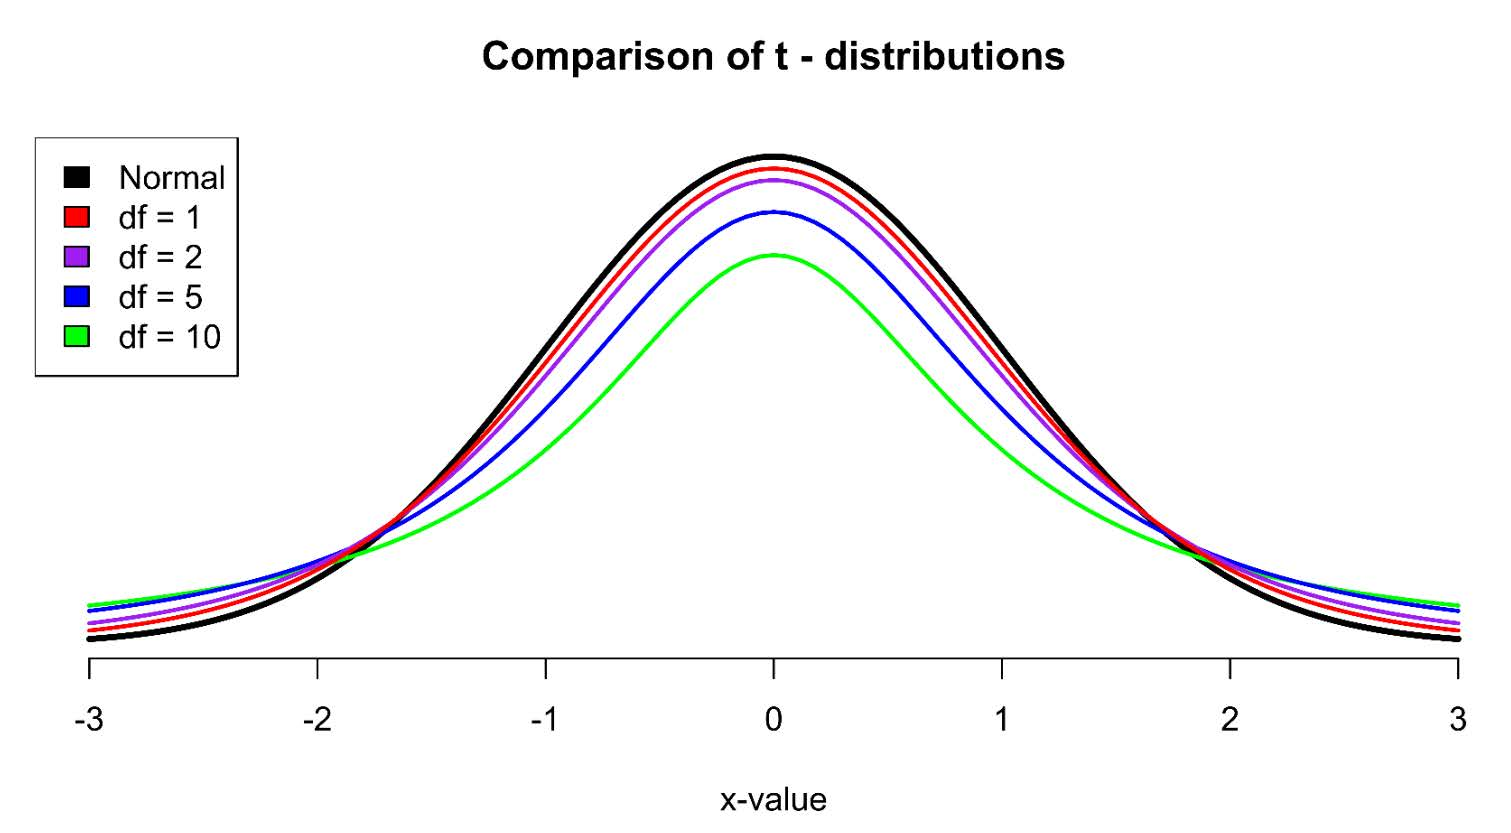
\includegraphics[width=.9\textwidth]{Files/Images/tdistributions.jpg}
\end{center}

Use the following \texttt{R} code to create a figure of the \concept{t-distribution} with $df = 3$. \\

\codeblock{curve(dnorm(x, mean = 0, sd = 1), from = -3, to = 3, ylab = \textquotesingle Density\textquotesingle)\\
curve(dt(x, df = 3), from = -3, to = 3, add = TRUE, col = \textquotesingle red\textquotesingle)
}

\question{
    Which line represents the \concept{normal distribution} in the figure that was drawn? And which line represents the \concept{t-distribution}? Can you explain what the difference between the two distributions is in terms of their shape? What happens when you increase the \concept{degrees of freedom} (\rcode{df}) in the \rcode{dt()} function?
}

\twolineanswerbox

\question{
    Calculate the \concept{degrees of freedom} and the \concept{t-value} for the \concept{correlation coefficient} between \rcode{Distance} and \rocde{AvgVisits}.
}

\hint{You can find the formula for the \concept{degrees of freedom} and the \concept{t-value} of a \concept{correlation} in the formula sheet on page~\pageref{formulasheet}.}

\clearpage % Page break

\rcodeanswertiny

\emptyanswerbox{
    $df$: \shortanswerline \hspace*{3cm} $t_{xy}$: \shortanswerline
}

\question{
    Where do you find the \concept{t-value} that you calculated in assignment 4.3e in the output of the \rcode{cor.test()} function from assignment 4.3c?
}

\onelineanswerbox

\question{
    What is the \concept{p-value} for this hypothesis test? Interpret this \concept{p-value} with respect to the confidence used and give a conclusion on the hypotheses. Include the following elements:
    \begin{itemize}
        \item[$\square$] Discuss what the \concept{p-value} is for this test.
    \item[$\square$] Discuss whether $H_0$ is rejected or not.
    \item[$\square$] Describe what this tells us about $\rho_{xy}$.  
    \item[$\square$] Describe what type of error is relevant \textit{(type-I or type-II)}.
\end{itemize}
}

\sixlineanswerbox

\clearpage % Page break